\documentclass[aspectratio=169]{beamer}
\usepackage{amsmath}
\usepackage{amssymb}
\usepackage{xcolor}
\usepackage{tikz}
\usetikzlibrary{positioning}

% ================================================================
% Quick Questions deck: solving equations.
%
% Each topic opens with five true/false statements and then runs ten
% quick questions that get gradually harder. Every question gets two
% slides: the question on its own for the mini whiteboards, then the
% same question again with the solution underneath in red.
%
% The three green topics are one step equations, then equations of
% the forms ax+b=c and x/a+b=c. The four amber topics are equations
% with the unknown on both sides, equations of the form (x+a)/b=c,
% constructing and solving equations, and equations with the unknown
% in the denominator. The two red topics are equations with algebraic
% fractions and simultaneous equations.
%
% The working is set out with the balance method: each line of the
% solution has a note beside it saying what was done to both sides.
% Where the working can be drawn it is: bar models drawn to scale at
% the solution for the one and two step equations, two bars of equal
% length for the unknown on both sides, function machines run
% forwards and then backwards for the two step equations (which also
% show why x/a+b=c and (x+a)/b=c are solved in a different order),
% the shapes and angles that the constructed equations come from, and
% graphs for simultaneous equations, where the solution is the point
% where the two lines cross.
% ================================================================

\setbeamertemplate{navigation symbols}{}

% A link in the bottom left of every slide back to the contents, so a
% deck this long can be jumped around in during a lesson.
\setbeamertemplate{footline}{%
  \hbox to\paperwidth{%
    \hspace{1em}%
    \hyperlink{contents}{%
      \color{gray}\scriptsize$\leftarrow$~Back to contents}%
    \hfil}%
  \vskip4pt%
}

% Topic divider.
\newcommand{\qtopic}[1]{%
  \section{#1}%
  \begin{frame}
    \vfill
    \begin{center}
      {\usebeamercolor[fg]{structure}\Huge\bfseries #1}
    \end{center}
    \vfill
  \end{frame}%
}

% \qq[<question size>][<solution size>]{<question>}{<solution>}
% The two optional sizes drop the type for the wordier questions and
% the longer solutions, so nothing runs off the slide.
\NewDocumentCommand{\qq}{O{\Huge}O{\LARGE}+m+m}{%
  \begin{frame}
    \vfill
    \begin{center}
      \begin{minipage}{0.92\textwidth}
        \centering #1 #3
      \end{minipage}
    \end{center}
    \vfill
  \end{frame}%
  \begin{frame}
    \vfill
    \begin{center}
      \begin{minipage}{0.92\textwidth}
        \centering #1 #3
        \par\vspace{0.9em}
        {\color{red}#2 #4}
      \end{minipage}
    \end{center}
    \vfill
  \end{frame}%
}

% \tf[<statement size>][<answer size>]{<statement>}{<answer>}
% As \qq, but with a standing "True or false?" heading above the
% statement. The statements hunt for the usual misconceptions, so the
% answer always says why, not just which.
\NewDocumentCommand{\tf}{O{\LARGE}O{\Large}+m+m}{%
  \begin{frame}
    \vfill
    \begin{center}
      \begin{minipage}{0.92\textwidth}
        \centering
        {\usebeamercolor[fg]{structure}\Large\bfseries True or false?}
        \par\vspace{1em}
        #1 #3
      \end{minipage}
    \end{center}
    \vfill
  \end{frame}%
  \begin{frame}
    \vfill
    \begin{center}
      \begin{minipage}{0.92\textwidth}
        \centering
        {\usebeamercolor[fg]{structure}\Large\bfseries True or false?}
        \par\vspace{1em}
        #1 #3
        \par\vspace{0.9em}
        {\color{red}#2 #4}
      \end{minipage}
    \end{center}
    \vfill
  \end{frame}%
}

% \steps{<rows>}: balance-method working, one equation per row with
% the equals signs lined up. Each row is
%   <left side> & <right side> & \by{<what was done to both sides>}
% and the first row leaves the note empty. \dfrac is taller than the
% row strut, so rows with a fraction carry an explicit skip such as
% \\[0.95em].
\newcommand{\steps}[1]{%
  \begin{tabular}{@{}r@{${}={}$}l@{\qquad}l@{}}#1\end{tabular}%
}
\newcommand{\by}[1]{{\normalsize #1}}

% \simwork{<rows>}: working for a pair of simultaneous equations. Each
% row is <label> & <left side> & <right side>, where the label numbers
% the equation or says how it was made from the numbered ones.
\newcommand{\simwork}[1]{%
  \begin{tabular}{@{}l@{\qquad}r@{${}={}$}l@{}}#1\end{tabular}%
}

% \side[<width of the left part>]{<left>}{<right>}
% Working and a diagram next to each other, for a solution that would
% be too tall with one above the other.
\NewDocumentCommand{\side}{O{0.5}+m+m}{%
  \begin{minipage}[c]{#1\linewidth}\centering #2\end{minipage}\hfill
  \begin{minipage}[c]{\dimexpr0.96\linewidth-#1\linewidth\relax}%
    \centering #3\end{minipage}%
}

% ================================================================
% Bar models
% ================================================================

% Each part of a bar is <size>/<label>/<fill>. The sizes are in the
% same units as the numbers in the equation, and the unknown is given
% its value at the solution, so every bar is drawn to scale. \bp is
% the plain fill; \bh is a darker fill for the parts that match up
% between two bars.
\def\bp{red!6}
\def\bh{red!28}

% \barrow{<y>}{<cm per unit>}{<parts>} draws one row of parts and
% leaves its total length in \barx.
\newcommand{\barrow}[3]{%
  \gdef\barx{0}%
  \foreach \v/\l/\f in {#3}{%
    \pgfmathsetmacro{\barnext}{\barx+\v*#2}%
    \draw[red!60!black, thick, fill=\f]
      (\barx,#1) rectangle (\barnext,#1+0.8);
    \node[red] at ({(\barx+\barnext)/2},#1+0.4) {$\l$};
    \xdef\barx{\barnext}}%
}

% \barmodel[<cm per unit>]{<total>}{<parts>}
% A bar split into parts, with the whole bar above it.
\newcommand{\barmodel}[3][0.5]{%
  \begin{tikzpicture}[font=\Large]
    \barrow{0}{#1}{#3}
    \draw[red!60!black, thick, fill=\bp] (0,0.95) rectangle (\barx,1.75);
    \node[red] at (\barx/2,1.35) {$#2$};
  \end{tikzpicture}%
}

% \barpair[<cm per unit>]{<top parts>}{<bottom parts>}
% Two bars of the same length, for the two sides of an equation with
% the unknown on both sides.
\newcommand{\barpair}[3][0.4]{%
  \begin{tikzpicture}[font=\Large]
    \barrow{0.95}{#1}{#2}
    \barrow{0}{#1}{#3}
  \end{tikzpicture}%
}

% ================================================================
% Function machines
% ================================================================

% \fmachine{<in>}{<op 1>}{<middle>}{<op 2>}{<out>}
%          {<answer>}{<inverse of op 1>}{<middle value>}{<inverse of op 2>}
% Top row: the equation as a function machine, with the unknown going
% in and the right-hand side coming out. Bottom row: the machine run
% backwards from the output, each operation replaced by its inverse,
% which gives the solution.
\tikzset{
  mbox/.style={draw=red!60!black, rounded corners=2pt, fill=red!8,
               inner sep=4pt, text=red, font=\Large,
               minimum width=1.3cm, minimum height=0.85cm},
  marr/.style={->, red, thick, shorten >=1pt, shorten <=1pt},
  mlab/.style={above, text=red, font=\large},
}
\newcommand{\fmachine}[9]{%
  \begin{tikzpicture}
    \node[mbox] (a1) at (0,0) {$#1$};
    \node[mbox] (a2) at (2.7,0) {$#3$};
    \node[mbox] (a3) at (5.4,0) {$#5$};
    \node[mbox] (b1) at (0,-1.45) {$#6$};
    \node[mbox] (b2) at (2.7,-1.45) {$#8$};
    \node[mbox] (b3) at (5.4,-1.45) {$#5$};
    \draw[marr] (a1) -- node[mlab]{$#2$} (a2);
    \draw[marr] (a2) -- node[mlab]{$#4$} (a3);
    \draw[marr] (b3) -- node[mlab]{$#9$} (b2);
    \draw[marr] (b2) -- node[mlab]{$#7$} (b1);
  \end{tikzpicture}%
}

% \fwd{<in>}{<op 1>}{<middle>}{<op 2>}{<out>}: the top row on its own,
% for comparing the order of the operations in two equations.
\newcommand{\fwd}[5]{%
  \begin{tikzpicture}[baseline=(a1.base)]
    \node[mbox] (a1) at (0,0) {$#1$};
    \node[mbox] (a2) at (2.7,0) {$#3$};
    \node[mbox] (a3) at (5.4,0) {$#5$};
    \draw[marr] (a1) -- node[mlab]{$#2$} (a2);
    \draw[marr] (a2) -- node[mlab]{$#4$} (a3);
  \end{tikzpicture}%
}

% Contents-slide bullets, colour-coded by difficulty band: green for
% the one and two step equations, orange for the four middle topics
% and red for algebraic fractions and simultaneous equations. The
% green is darkened because a pure green washes out on a projector.
\setbeamertemplate{section in toc}{%
  \ifnum\inserttocsectionnumber<4
    \textcolor{green!55!black}{$\bullet$}%
  \else
    \ifnum\inserttocsectionnumber<8
      \textcolor{orange}{$\bullet$}%
    \else
      \textcolor{red}{$\bullet$}%
    \fi
  \fi
  ~\inserttocsection%
}

\title{Solving Equations: Quick Questions}
\subtitle{Mini whiteboard questions, with solutions}
\author{}
\date{}

\begin{document}

\frame{\titlepage}

\begin{frame}[label=contents]{Contents}
  \small
  \tableofcontents
\end{frame}

%================================================================
\qtopic{One step equations}
%================================================================

\tf{The solution of $x+6=10$ is $x=16$}
  {\textbf{False.} $16+6=22$, not $10$.
   \par\vspace{0.4em}
   \steps{$x+6$ & $10$ & \\
          $x$ & $4$ & \by{subtract $6$ from both sides}}
   \par\vspace{0.5em}
   \barmodel[0.55]{10}{4/x/\bp,6/6/\bp}}

\tf{$4x=20$, so $x=5$}
  {\textbf{True.} $4x$ means $4\times x$, so we divide both sides by $4$.\\[0.3em]
   Check: $4\times 5=20$
   \par\vspace{0.5em}
   \barmodel[0.3]{20}{5/x/\bp,5/x/\bp,5/x/\bp,5/x/\bp}}

\tf{To solve $x-3=9$ we subtract $3$ from both sides}
  {\textbf{False.} The inverse of subtracting $3$ is adding $3$.
   \par\vspace{0.4em}
   \steps{$x-3$ & $9$ & \\
          $x$ & $12$ & \by{add $3$ to both sides}}
   \par\vspace{0.5em}
   \barmodel[0.45]{x}{9/9/\bp,3/3/\bp}}

\tf{The solution of $\dfrac{x}{2}=8$ is $x=4$}
  {\textbf{False.} $\dfrac{x}{2}$ means $x\div 2$, and $4\div 2=2$, not $8$.
   \par\vspace{0.4em}
   \steps{$\dfrac{x}{2}$ & $8$ & \\[0.95em]
          $x$ & $16$ & \by{multiply both sides by $2$}}
   \par\vspace{0.5em}
   \barmodel[0.35]{x}{8/8/\bp,8/8/\bp}}

\tf{The solution of $15=x+9$ is $x=6$}
  {\textbf{True.} The unknown can be on either side of the equals sign.\\[0.3em]
   \steps{$15$ & $x+9$ & \\
          $6$ & $x$ & \by{subtract $9$ from both sides}}\\[0.3em]
   $6=x$ is the same as $x=6$.}

\qq{Solve $x+5=12$}
  {\steps{$x+5$ & $12$ & \\
          $x$ & $7$ & \by{subtract $5$ from both sides}}
   \par\vspace{0.6em}
   \barmodel[0.5]{12}{7/x/\bp,5/5/\bp}}

\qq{Solve $x-4=11$}
  {\steps{$x-4$ & $11$ & \\
          $x$ & $15$ & \by{add $4$ to both sides}}
   \par\vspace{0.6em}
   \barmodel[0.4]{x}{11/11/\bp,4/4/\bp}}

\qq{Solve $3x=21$}
  {\steps{$3x$ & $21$ & \\
          $x$ & $7$ & \by{divide both sides by $3$}}
   \par\vspace{0.6em}
   \barmodel[0.3]{21}{7/x/\bp,7/x/\bp,7/x/\bp}}

\qq{Solve $\dfrac{x}{5}=6$}
  {\steps{$\dfrac{x}{5}$ & $6$ & \\[0.95em]
          $x$ & $30$ & \by{multiply both sides by $5$}}
   \par\vspace{0.6em}
   \barmodel[0.2]{x}{6/6/\bp,6/6/\bp,6/6/\bp,6/6/\bp,6/6/\bp}}

\qq{Solve $x+13=8$}
  {\steps{$x+13$ & $8$ & \\
          $x$ & $-5$ & \by{subtract $13$ from both sides}}\\[0.4em]
   Check: $-5+13=8$}

\qq{Solve $5x=8$}
  {\steps{$5x$ & $8$ & \\[0.3em]
          $x$ & $\dfrac{8}{5}=1.6$ & \by{divide both sides by $5$}}\\[0.5em]
   The solution does not have to be a whole number.}

\qq{Solve $-3x=18$}
  {\steps{$-3x$ & $18$ & \\
          $x$ & $-6$ & \by{divide both sides by $-3$}}\\[0.4em]
   Check: $-3\times(-6)=18$}

\qq{Solve $\dfrac{x}{4}=-7$}
  {\steps{$\dfrac{x}{4}$ & $-7$ & \\[0.95em]
          $x$ & $-28$ & \by{multiply both sides by $4$}}\\[0.4em]
   Check: $-28\div 4=-7$}

\qq{Solve $12-x=5$}
  {\steps{$12-x$ & $5$ & \\
          $12$ & $5+x$ & \by{add $x$ to both sides}\\
          $7$ & $x$ & \by{subtract $5$ from both sides}}
   \par\vspace{0.6em}
   \barmodel[0.5]{12}{7/x/\bp,5/5/\bp}}

\qq[\LARGE][\Large]{$6$ identical notebooks cost \pounds$8.40$ in total.\\[0.3em]
   Write an equation for the cost, \pounds$c$, of one notebook,\\[0.1em]
   and solve it.}
  {\side[0.55]{\steps{$6c$ & $8.40$ & \\
                      $c$ & $1.40$ & \by{divide by $6$}}\\[0.4em]
               One notebook costs \pounds$1.40$.}
     {\barmodel[0.6]{8.40}{1.4/c/\bp,1.4/c/\bp,1.4/c/\bp,1.4/c/\bp,1.4/c/\bp,1.4/c/\bp}}}

%================================================================
\qtopic{Equations of the form \texorpdfstring{$ax+b=c$}{ax+b=c}}
%================================================================

\tf{$2x+5=17$ gives $2x=12$, so $x=10$}
  {\textbf{False.} $2x$ means $2\times x$, so we divide by $2$, not
   subtract $2$.
   \par\vspace{0.4em}
   \steps{$2x+5$ & $17$ & \\
          $2x$ & $12$ & \by{subtract $5$ from both sides}\\
          $x$ & $6$ & \by{divide both sides by $2$}}\\[0.4em]
   Check: $2\times 6+5=17$}

\tf{$3x-4=11$ and $3x=15$ have the same solution}
  {\textbf{True.} Adding $4$ to both sides of $3x-4=11$ gives $3x=15$.\\
   Doing the same to both sides keeps them equal,\\
   so the solution does not change.
   \par\vspace{0.4em}
   \steps{$3x-4$ & $11$ & \\
          $3x$ & $15$ & \by{add $4$ to both sides}\\
          $x$ & $5$ & \by{divide both sides by $3$}}\\[0.4em]
   Check: $3\times 5-4=11$ and $3\times 5=15$}

\tf{Dividing both sides of $4x+3=23$ by $4$ gives\\[0.3em]
   $x+3=\dfrac{23}{4}$}
  {\textbf{False.} Every term is divided by $4$, including the $3$:\\[0.3em]
   $x+\dfrac{3}{4}=\dfrac{23}{4}$\\[0.4em]
   It is simpler to subtract $3$ first: $4x=20$, so $x=5$.}

\tf{The solution of $5x+2=2$ is $x=0$}
  {\textbf{True.}
   \par\vspace{0.4em}
   \steps{$5x+2$ & $2$ & \\
          $5x$ & $0$ & \by{subtract $2$ from both sides}\\
          $x$ & $0$ & \by{divide both sides by $5$}}\\[0.4em]
   Check: $5\times 0+2=2$}

\tf{The solution of an equation is always a whole number}
  {\textbf{False.} For example,
   \par\vspace{0.3em}
   \steps{$2x+1$ & $4$ & \\
          $2x$ & $3$ & \by{subtract $1$ from both sides}\\
          $x$ & $1.5$ & \by{divide both sides by $2$}}}

\qq[\Huge][\Large]{Solve $2x+3=11$}
  {\steps{$2x+3$ & $11$ & \\
          $2x$ & $8$ & \by{subtract $3$ from both sides}\\
          $x$ & $4$ & \by{divide both sides by $2$}}
   \par\vspace{0.6em}
   \barmodel[0.5]{11}{4/x/\bp,4/x/\bp,3/3/\bp}}

\qq[\Huge][\Large]{Solve $3x+5=26$}
  {\side[0.42]{\steps{$3x+5$ & $26$ & \\
                      $3x$ & $21$ & \by{subtract $5$}\\
                      $x$ & $7$ & \by{divide by $3$}}}
     {\fmachine{x}{\times 3}{3x}{+5}{26}{7}{\div 3}{21}{-5}}}

\qq[\Huge][\Large]{Solve $4x-7=25$}
  {\steps{$4x-7$ & $25$ & \\
          $4x$ & $32$ & \by{add $7$ to both sides}\\
          $x$ & $8$ & \by{divide both sides by $4$}}\\[0.4em]
   Check: $4\times 8-7=25$}

\qq[\Huge][\Large]{Solve $23=5x+8$}
  {\steps{$23$ & $5x+8$ & \\
          $15$ & $5x$ & \by{subtract $8$ from both sides}\\
          $3$ & $x$ & \by{divide both sides by $5$}}\\[0.4em]
   The solution is $x=3$.}

\qq[\Huge][\Large]{Solve $5x+9=4$}
  {\steps{$5x+9$ & $4$ & \\
          $5x$ & $-5$ & \by{subtract $9$ from both sides}\\
          $x$ & $-1$ & \by{divide both sides by $5$}}\\[0.4em]
   Check: $5\times(-1)+9=4$}

\qq[\Huge][\Large]{Solve $6x-1=14$}
  {\steps{$6x-1$ & $14$ & \\[0.3em]
          $6x$ & $15$ & \by{add $1$ to both sides}\\[0.3em]
          $x$ & $\dfrac{15}{6}=2.5$ & \by{divide both sides by $6$}}}

\qq[\Huge][\Large]{Solve $10-2x=4$}
  {Adding $2x$ to both sides makes the $x$ term positive.
   \par\vspace{0.4em}
   \steps{$10-2x$ & $4$ & \\
          $10$ & $4+2x$ & \by{add $2x$ to both sides}\\
          $6$ & $2x$ & \by{subtract $4$ from both sides}\\
          $3$ & $x$ & \by{divide both sides by $2$}}}

\qq[\Huge][\Large]{Solve $8x+13=7$}
  {\steps{$8x+13$ & $7$ & \\[0.3em]
          $8x$ & $-6$ & \by{subtract $13$ from both sides}\\[0.3em]
          $x$ & $-\dfrac{6}{8}=-0.75$ & \by{divide both sides by $8$}}\\[0.4em]
   Check: $8\times(-0.75)+13=-6+13=7$}

\qq[\Huge][\Large]{Solve $0.4x+1=3$}
  {\steps{$0.4x+1$ & $3$ & \\[0.3em]
          $0.4x$ & $2$ & \by{subtract $1$ from both sides}\\[0.3em]
          $x$ & $\dfrac{2}{0.4}=\dfrac{20}{4}=5$ & \by{divide both sides by $0.4$}}}

\qq[\LARGE][\Large]{A taxi charges \pounds$3$, plus \pounds$2$ for every mile.\\[0.3em]
   A journey costs \pounds$19$.\\[0.3em]
   How many miles long is the journey?}
  {We write $m$ for the length of the journey in miles.
   \par\vspace{0.3em}
   \side[0.54]{\steps{$2m+3$ & $19$ & \\
                      $2m$ & $16$ & \by{subtract $3$}\\
                      $m$ & $8$ & \by{divide by $2$}}\\[0.4em]
               The journey is $8$ miles long.}
     {\barmodel[0.25]{19}{8/m/\bp,8/m/\bp,3/3/\bp}}}

%================================================================
\qtopic{Equations of the form \texorpdfstring{$\frac{x}{a}+b=c$}{x/a+b=c}}
%================================================================

\tf[\LARGE][\large]{To solve $\dfrac{x}{3}+2=5$, we subtract $2$\\[0.3em]
   before we multiply by $3$}
  {\textbf{True.} $x$ is divided by $3$ and then $2$ is added, so the
   inverse operations are done in the reverse order.
   \par\vspace{0.4em}
   \steps{$\dfrac{x}{3}+2$ & $5$ & \\[0.95em]
          $\dfrac{x}{3}$ & $3$ & \by{subtract $2$ from both sides}\\[0.95em]
          $x$ & $9$ & \by{multiply both sides by $3$}}}

\tf{Multiplying both sides of $\dfrac{x}{4}+1=6$ by $4$ gives\\[0.3em]
   $x+1=24$}
  {\textbf{False.} Every term is multiplied by $4$, including the $1$.
   \par\vspace{0.4em}
   \steps{$\dfrac{x}{4}+1$ & $6$ & \\[0.95em]
          $x+4$ & $24$ & \by{multiply every term by $4$}\\
          $x$ & $20$ & \by{subtract $4$ from both sides}}}

\tf{The solution of $\dfrac{x}{5}-2=3$ is $x=5$}
  {\textbf{False.} $5$ is the value of $\dfrac{x}{5}$, not of $x$.
   \par\vspace{0.4em}
   \steps{$\dfrac{x}{5}-2$ & $3$ & \\[0.95em]
          $\dfrac{x}{5}$ & $5$ & \by{add $2$ to both sides}\\[0.95em]
          $x$ & $25$ & \by{multiply both sides by $5$}}}

\tf{$\dfrac{x}{2}+3$ means divide $x$ by $2$, then add $3$}
  {\textbf{True.} The fraction bar is only under the $x$,\\
   so the division comes first.
   \par\vspace{0.5em}
   \fwd{x}{\div 2}{\dfrac{x}{2}}{+3}{\dfrac{x}{2}+3}\\[0.5em]
   $\dfrac{x+3}{2}$ would mean add $3$ first, then divide by $2$.}

\tf{$\dfrac{x}{6}+4=1$ has no solution,\\[0.3em] because $1$ is less than $4$}
  {\textbf{False.} The solution is a negative number.
   \par\vspace{0.4em}
   \steps{$\dfrac{x}{6}+4$ & $1$ & \\[0.95em]
          $\dfrac{x}{6}$ & $-3$ & \by{subtract $4$ from both sides}\\[0.95em]
          $x$ & $-18$ & \by{multiply both sides by $6$}}}

\qq[\Huge][\Large]{Solve $\dfrac{x}{2}+3=7$}
  {\side[0.42]{\steps{$\dfrac{x}{2}+3$ & $7$ & \\[0.95em]
                      $\dfrac{x}{2}$ & $4$ & \by{subtract $3$}\\[0.95em]
                      $x$ & $8$ & \by{multiply by $2$}}}
     {\fmachine{x}{\div 2}{\dfrac{x}{2}}{+3}{7}{8}{\times 2}{4}{-3}}}

\qq[\Huge][\Large]{Solve $\dfrac{x}{4}+5=8$}
  {\steps{$\dfrac{x}{4}+5$ & $8$ & \\[0.95em]
          $\dfrac{x}{4}$ & $3$ & \by{subtract $5$ from both sides}\\[0.95em]
          $x$ & $12$ & \by{multiply both sides by $4$}}
   \par\vspace{0.6em}
   \barmodel[0.45]{x}{3/3/\bp,3/3/\bp,3/3/\bp,3/3/\bp}}

\qq[\Huge][\Large]{Solve $\dfrac{x}{3}-2=5$}
  {\steps{$\dfrac{x}{3}-2$ & $5$ & \\[0.95em]
          $\dfrac{x}{3}$ & $7$ & \by{add $2$ to both sides}\\[0.95em]
          $x$ & $21$ & \by{multiply both sides by $3$}}}

\qq[\Huge][\Large]{Solve $10=\dfrac{x}{3}+4$}
  {\steps{$10$ & $\dfrac{x}{3}+4$ & \\[0.95em]
          $6$ & $\dfrac{x}{3}$ & \by{subtract $4$ from both sides}\\[0.95em]
          $18$ & $x$ & \by{multiply both sides by $3$}}}

\qq[\Huge][\Large]{Solve $\dfrac{x}{2}+9=4$}
  {\steps{$\dfrac{x}{2}+9$ & $4$ & \\[0.95em]
          $\dfrac{x}{2}$ & $-5$ & \by{subtract $9$ from both sides}\\[0.95em]
          $x$ & $-10$ & \by{multiply both sides by $2$}}}

\qq[\Huge][\Large]{Solve $\dfrac{x}{4}-1.5=2$}
  {\steps{$\dfrac{x}{4}-1.5$ & $2$ & \\[0.95em]
          $\dfrac{x}{4}$ & $3.5$ & \by{add $1.5$ to both sides}\\[0.95em]
          $x$ & $14$ & \by{multiply both sides by $4$}}}

\qq[\Huge][\Large]{Solve $\dfrac{2x}{5}+1=7$}
  {\steps{$\dfrac{2x}{5}+1$ & $7$ & \\[0.95em]
          $\dfrac{2x}{5}$ & $6$ & \by{subtract $1$ from both sides}\\[0.95em]
          $2x$ & $30$ & \by{multiply both sides by $5$}\\
          $x$ & $15$ & \by{divide both sides by $2$}}}

\qq[\Huge][\Large]{Solve $\dfrac{2x}{3}+5=1$}
  {\steps{$\dfrac{2x}{3}+5$ & $1$ & \\[0.95em]
          $\dfrac{2x}{3}$ & $-4$ & \by{subtract $5$ from both sides}\\[0.95em]
          $2x$ & $-12$ & \by{multiply both sides by $3$}\\
          $x$ & $-6$ & \by{divide both sides by $2$}}}

\qq[\Huge][\Large]{Solve $6-\dfrac{x}{3}=2$}
  {\steps{$6-\dfrac{x}{3}$ & $2$ & \\[0.95em]
          $6$ & $2+\dfrac{x}{3}$ & \by{add $\dfrac{x}{3}$ to both sides}\\[0.95em]
          $4$ & $\dfrac{x}{3}$ & \by{subtract $2$ from both sides}\\[0.95em]
          $12$ & $x$ & \by{multiply both sides by $3$}}}

\qq[\Large][\Large]{Four friends share the cost of a meal equally.\\[0.3em]
   Each friend also pays \pounds$3$ for a drink.\\[0.3em]
   Each friend pays \pounds$17$ in total.\\[0.3em]
   How much did the meal cost?}
  {We write \pounds$m$ for the cost of the meal.
   \par\vspace{0.3em}
   \side[0.55]{\steps{$\dfrac{m}{4}+3$ & $17$ & \\[0.95em]
                      $\dfrac{m}{4}$ & $14$ & \by{subtract $3$}\\[0.95em]
                      $m$ & $56$ & \by{multiply by $4$}}\\[0.4em]
               The meal cost \pounds$56$.}
     {\barmodel[0.09]{m}{14/14/\bp,14/14/\bp,14/14/\bp,14/14/\bp}}}

%================================================================
\qtopic{Equations with the unknown on both sides}
%================================================================

\tf{To solve $5x+2=3x+10$,\\[0.3em] we can subtract $3x$ from both sides}
  {\textbf{True.} This leaves the $x$ terms on one side only.
   \par\vspace{0.4em}
   \steps{$5x+2$ & $3x+10$ & \\
          $2x+2$ & $10$ & \by{subtract $3x$ from both sides}\\
          $2x$ & $8$ & \by{subtract $2$ from both sides}\\
          $x$ & $4$ & \by{divide both sides by $2$}}}

\tf{Solving $4x+1=2x+7$, the first step gives\\[0.3em] $6x+1=7$}
  {\textbf{False.} $6x+1=7$ comes from adding $2x$ on the left\\
   but subtracting $2x$ on the right.\\
   We must do the same to both sides.
   \par\vspace{0.4em}
   \steps{$4x+1$ & $2x+7$ & \\
          $2x+1$ & $7$ & \by{subtract $2x$ from both sides}\\
          $2x$ & $6$ & \by{subtract $1$ from both sides}\\
          $x$ & $3$ & \by{divide both sides by $2$}}}

\tf{$3x+5=3x+8$ has no solution}
  {\textbf{True.} Subtracting $3x$ from both sides gives $5=8$.\\[0.3em]
   $5=8$ is never true, so no value of $x$ works.}

\tf{Solving $7x-3=2x+12$ gives $5x=9$}
  {\textbf{False.} Subtracting $2x$ from both sides gives $5x-3=12$. The
   inverse of subtracting $3$ is adding $3$, so $5x=15$, not $9$.
   \par\vspace{0.4em}
   \steps{$7x-3$ & $2x+12$ & \\
          $5x-3$ & $12$ & \by{subtract $2x$ from both sides}\\
          $5x$ & $15$ & \by{add $3$ to both sides}\\
          $x$ & $3$ & \by{divide both sides by $5$}}}

\tf{In $2x+9=6x+1$ the $x$ terms must be collected\\[0.3em]
   on the left-hand side}
  {\textbf{False.} Collecting them on the right, where there are more,
   keeps the $x$ term positive.
   \par\vspace{0.4em}
   \steps{$2x+9$ & $6x+1$ & \\
          $9$ & $4x+1$ & \by{subtract $2x$ from both sides}\\
          $8$ & $4x$ & \by{subtract $1$ from both sides}\\
          $2$ & $x$ & \by{divide both sides by $4$}}}

\qq[\Huge][\Large]{Solve $5x+3=2x+15$}
  {\steps{$5x+3$ & $2x+15$ & \\
          $3x+3$ & $15$ & \by{subtract $2x$ from both sides}\\
          $3x$ & $12$ & \by{subtract $3$ from both sides}\\
          $x$ & $4$ & \by{divide both sides by $3$}}
   \par\vspace{0.4em}
   The two bars are the same length.\\
   We subtract the shaded $2x$ from both bars.
   \par\vspace{0.3em}
   \barpair[0.3]{4/x/\bh,4/x/\bh,4/x/\bp,4/x/\bp,4/x/\bp,3/3/\bp}
                {4/x/\bh,4/x/\bh,15/15/\bp}}

\qq[\Huge][\Large]{Solve $6x+1=4x+13$}
  {\steps{$6x+1$ & $4x+13$ & \\
          $2x+1$ & $13$ & \by{subtract $4x$ from both sides}\\
          $2x$ & $12$ & \by{subtract $1$ from both sides}\\
          $x$ & $6$ & \by{divide both sides by $2$}}}

\qq[\Huge][\Large]{Solve $7x-2=3x+10$}
  {\steps{$7x-2$ & $3x+10$ & \\
          $4x-2$ & $10$ & \by{subtract $3x$ from both sides}\\
          $4x$ & $12$ & \by{add $2$ to both sides}\\
          $x$ & $3$ & \by{divide both sides by $4$}}}

\qq[\Huge][\Large]{Solve $4x+9=x-3$}
  {\steps{$4x+9$ & $x-3$ & \\
          $3x+9$ & $-3$ & \by{subtract $x$ from both sides}\\
          $3x$ & $-12$ & \by{subtract $9$ from both sides}\\
          $x$ & $-4$ & \by{divide both sides by $3$}}}

\qq[\Huge][\Large]{Solve $2x+17=5x+2$}
  {There are more $x$ terms on the right, so we collect them there.
   \par\vspace{0.4em}
   \steps{$2x+17$ & $5x+2$ & \\
          $17$ & $3x+2$ & \by{subtract $2x$ from both sides}\\
          $15$ & $3x$ & \by{subtract $2$ from both sides}\\
          $5$ & $x$ & \by{divide both sides by $3$}}}

\qq[\Huge][\Large]{Solve $5x-4=2x+7$}
  {\steps{$5x-4$ & $2x+7$ & \\[0.2em]
          $3x-4$ & $7$ & \by{subtract $2x$ from both sides}\\[0.2em]
          $3x$ & $11$ & \by{add $4$ to both sides}\\[0.2em]
          $x$ & $\dfrac{11}{3}=3\dfrac{2}{3}$ & \by{divide both sides by $3$}}}

\qq[\Huge][\Large]{Solve $14-x=3x-2$}
  {\steps{$14-x$ & $3x-2$ & \\
          $14$ & $4x-2$ & \by{add $x$ to both sides}\\
          $16$ & $4x$ & \by{add $2$ to both sides}\\
          $4$ & $x$ & \by{divide both sides by $4$}}}

\qq[\Huge][\Large]{Solve $3(x+2)=x+18$}
  {\steps{$3(x+2)$ & $x+18$ & \\
          $3x+6$ & $x+18$ & \by{expand the bracket}\\
          $2x+6$ & $18$ & \by{subtract $x$ from both sides}\\
          $2x$ & $12$ & \by{subtract $6$ from both sides}\\
          $x$ & $6$ & \by{divide both sides by $2$}}}

\qq[\Huge][\Large]{Solve $4(2x-1)=3(x+2)$}
  {\steps{$4(2x-1)$ & $3(x+2)$ & \\
          $8x-4$ & $3x+6$ & \by{expand the brackets}\\
          $5x-4$ & $6$ & \by{subtract $3x$ from both sides}\\
          $5x$ & $10$ & \by{add $4$ to both sides}\\
          $x$ & $2$ & \by{divide both sides by $5$}}}

\qq[\Large][\Large]{Ali has \pounds$40$ and saves \pounds$5$ a week.\\[0.3em]
   Bea has \pounds$16$ and saves \pounds$8$ a week.\\[0.3em]
   After how many weeks will they\\[0.1em] have the same amount?}
  {We write $w$ for the number of weeks.
   \par\vspace{0.3em}
   \steps{$40+5w$ & $16+8w$ & \\
          $24+5w$ & $8w$ & \by{subtract $16$ from both sides}\\
          $24$ & $3w$ & \by{subtract $5w$ from both sides}\\
          $8$ & $w$ & \by{divide both sides by $3$}}\\[0.4em]
   After $8$ weeks they both have \pounds$80$.}

%================================================================
\qtopic{Equations of the form \texorpdfstring{$\frac{x+a}{b}=c$}{(x+a)/b=c}}
%================================================================

\tf{$\dfrac{x+2}{3}=5$ and $\dfrac{x}{3}+2=5$ have the same solution}
  {\textbf{False.} The operations are done in a different order.
   \par\vspace{0.5em}
   \begin{tabular}{@{}c@{\qquad}l@{}}
     \fwd{x}{+2}{x+2}{\div 3}{5} & $x=13$\\[0.5em]
     \fwd{x}{\div 3}{\dfrac{x}{3}}{+2}{5} & $x=9$
   \end{tabular}}

\tf{To solve $\dfrac{x+4}{2}=7$, we can start by\\[0.3em]
   multiplying both sides by $2$}
  {\textbf{True.} The whole of $x+4$ is divided by $2$,\\
   so we multiply both sides by $2$ first.
   \par\vspace{0.4em}
   \steps{$\dfrac{x+4}{2}$ & $7$ & \\[0.95em]
          $x+4$ & $14$ & \by{multiply both sides by $2$}\\
          $x$ & $10$ & \by{subtract $4$ from both sides}}}

\tf{The solution of $\dfrac{x-1}{4}=3$ is $x=16$}
  {\textbf{False.} $16$ comes from adding $1$ before multiplying by $4$,
   which is the wrong order.
   \par\vspace{0.4em}
   \steps{$\dfrac{x-1}{4}$ & $3$ & \\[0.95em]
          $x-1$ & $12$ & \by{multiply both sides by $4$}\\
          $x$ & $13$ & \by{add $1$ to both sides}}\\[0.4em]
   Check: $(13-1)\div 4=3$, but $(16-1)\div 4=3.75$}

\tf{$\dfrac{x+6}{3}=4$ simplifies to $x+2=4$}
  {\textbf{False.} The $3$ divides the whole of $x+6$, not only the $6$.
   \par\vspace{0.4em}
   \steps{$\dfrac{x+6}{3}$ & $4$ & \\[0.95em]
          $x+6$ & $12$ & \by{multiply both sides by $3$}\\
          $x$ & $6$ & \by{subtract $6$ from both sides}}\\[0.4em]
   Check: $\dfrac{6+6}{3}=4$, but $x=2$ gives $\dfrac{2+6}{3}=\dfrac{8}{3}$}

\tf{The solution of $\dfrac{2x+1}{5}=3$ is $x=7$}
  {\textbf{True.} Check: $\dfrac{2\times 7+1}{5}=\dfrac{15}{5}=3$
   \par\vspace{0.4em}
   \steps{$\dfrac{2x+1}{5}$ & $3$ & \\[0.95em]
          $2x+1$ & $15$ & \by{multiply both sides by $5$}\\
          $2x$ & $14$ & \by{subtract $1$ from both sides}\\
          $x$ & $7$ & \by{divide both sides by $2$}}}

\qq[\Huge][\Large]{Solve $\dfrac{x+3}{2}=5$}
  {\side[0.44]{\steps{$\dfrac{x+3}{2}$ & $5$ & \\[0.95em]
                      $x+3$ & $10$ & \by{multiply by $2$}\\
                      $x$ & $7$ & \by{subtract $3$}}}
     {\fmachine{x}{+3}{x+3}{\div 2}{5}{7}{-3}{10}{\times 2}}}

\qq[\Huge][\Large]{Solve $\dfrac{x-4}{3}=2$}
  {\steps{$\dfrac{x-4}{3}$ & $2$ & \\[0.95em]
          $x-4$ & $6$ & \by{multiply both sides by $3$}\\
          $x$ & $10$ & \by{add $4$ to both sides}}}

\qq[\Huge][\Large]{Solve $\dfrac{x+1}{4}=3$}
  {\steps{$\dfrac{x+1}{4}$ & $3$ & \\[0.95em]
          $x+1$ & $12$ & \by{multiply both sides by $4$}\\
          $x$ & $11$ & \by{subtract $1$ from both sides}}}

\qq[\Huge][\Large]{Solve $\dfrac{x+8}{5}=1$}
  {\steps{$\dfrac{x+8}{5}$ & $1$ & \\[0.95em]
          $x+8$ & $5$ & \by{multiply both sides by $5$}\\
          $x$ & $-3$ & \by{subtract $8$ from both sides}}}

\qq[\Huge][\Large]{Solve $6=\dfrac{x-2}{3}$}
  {\steps{$6$ & $\dfrac{x-2}{3}$ & \\[0.95em]
          $18$ & $x-2$ & \by{multiply both sides by $3$}\\
          $20$ & $x$ & \by{add $2$ to both sides}}}

\qq[\Huge][\Large]{Solve $\dfrac{2x+3}{5}=3$}
  {\steps{$\dfrac{2x+3}{5}$ & $3$ & \\[0.95em]
          $2x+3$ & $15$ & \by{multiply both sides by $5$}\\
          $2x$ & $12$ & \by{subtract $3$ from both sides}\\
          $x$ & $6$ & \by{divide both sides by $2$}}}

\qq[\Huge][\Large]{Solve $\dfrac{3x-1}{4}=5$}
  {\steps{$\dfrac{3x-1}{4}$ & $5$ & \\[0.95em]
          $3x-1$ & $20$ & \by{multiply both sides by $4$}\\
          $3x$ & $21$ & \by{add $1$ to both sides}\\
          $x$ & $7$ & \by{divide both sides by $3$}}}

\qq[\Huge][\Large]{Solve $\dfrac{3x+7}{2}=-4$}
  {\steps{$\dfrac{3x+7}{2}$ & $-4$ & \\[0.95em]
          $3x+7$ & $-8$ & \by{multiply both sides by $2$}\\
          $3x$ & $-15$ & \by{subtract $7$ from both sides}\\
          $x$ & $-5$ & \by{divide both sides by $3$}}}

\qq[\Huge][\Large]{Solve $\dfrac{5x+2}{3}=x+2$}
  {The whole of the right-hand side is multiplied by $3$,\\
   so we write it in brackets.
   \par\vspace{0.4em}
   \steps{$\dfrac{5x+2}{3}$ & $x+2$ & \\[0.95em]
          $5x+2$ & $3(x+2)$ & \by{multiply both sides by $3$}\\
          $5x+2$ & $3x+6$ & \by{expand the bracket}\\
          $2x$ & $4$ & \by{subtract $3x$ and $2$ from both sides}\\
          $x$ & $2$ & \by{divide both sides by $2$}}}

\qq[\LARGE][\Large]{The mean of the three numbers $x$, $7$ and $10$ is $9$.\\[0.4em]
   Find $x$.}
  {The mean is the total divided by how many numbers there are.
   \par\vspace{0.4em}
   \steps{$\dfrac{x+7+10}{3}$ & $9$ & \\[0.95em]
          $\dfrac{x+17}{3}$ & $9$ & \by{collect like terms}\\[0.95em]
          $x+17$ & $27$ & \by{multiply both sides by $3$}\\
          $x$ & $10$ & \by{subtract $17$ from both sides}}}

%================================================================
\qtopic{Constructing and solving equations}
%================================================================

\tf[\Large][\Large]{``I think of a number, double it and add $5$.
   The answer is $17$.''\\[0.4em]
   This gives the equation $2(n+5)=17$}
  {\textbf{False.} The number is doubled first, so the equation is
   $2n+5=17$.
   \par\vspace{0.4em}
   \fwd{n}{\times 2}{2n}{+5}{17}\\[0.4em]
   $2(n+5)$ would mean add $5$ first, then double. Solving $2n+5=17$
   gives $n=6$.}

\tf[\Large][\Large]{The angles in this triangle give the equation\\[0.3em]
   $x+2x+3x=180$\\[0.5em]
   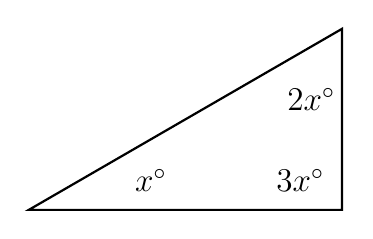
\begin{tikzpicture}[scale=1.15, font=\large]
     \draw[thick] (0,0) -- (3.46,0) -- (3.46,2) -- cycle;
     \node at (1.35,0.33) {$x^{\circ}$};
     \node at (3.0,0.33) {$3x^{\circ}$};
     \node at (3.12,1.22) {$2x^{\circ}$};
   \end{tikzpicture}}
  {\textbf{True.} The angles in a triangle add up to $180^{\circ}$.\\[0.3em]
   $6x=180$, so $x=30$ and the angles are $30^{\circ}$, $60^{\circ}$ and
   $90^{\circ}$.}

\tf[\Large][\Large]{The perimeter of this rectangle is $28$\,cm,\\[0.3em]
   so $x+4+x=28$\\[0.5em]
   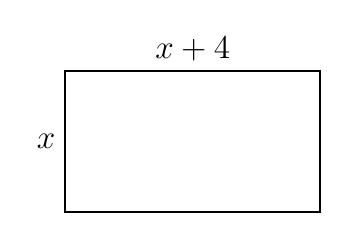
\begin{tikzpicture}[x=0.36cm, y=0.36cm, font=\large]
     \draw[thick] (0,0) rectangle (9,5);
     \node[above] at (4.5,5) {$x+4$};
     \node[left] at (0,2.5) {$x$};
   \end{tikzpicture}}
  {\textbf{False.} The perimeter is the total length of all four sides.\\[0.3em]
   $(x+4)+x+(x+4)+x=28$, so $4x+8=28$ and $x=5$.}

\tf[\Large][\Large]{Three consecutive integers add up to $48$.\\[0.3em]
   If the smallest is $n$, then $n+(n+1)+(n+2)=48$}
  {\textbf{True.} Each integer is $1$ more than the one before.\\[0.3em]
   $3n+3=48$, so $3n=45$ and $n=15$.\\[0.3em]
   The integers are $15$, $16$ and $17$.}

\tf{Jo is $3$ years older than Ken.\\[0.3em]
   If Ken is $k$ years old, then Jo is $3k$ years old}
  {\textbf{False.} $3k$ means $3\times k$, which is three times Ken's age.\\[0.3em]
   Jo is $3$ years older, so Jo is $k+3$ years old.}

\qq[\LARGE][\Large]{I think of a number, multiply it by $3$ and subtract $4$.\\[0.3em]
   The answer is $20$. What is my number?}
  {We write $n$ for my number.
   \par\vspace{0.3em}
   \side[0.42]{\steps{$3n-4$ & $20$ & \\
                      $3n$ & $24$ & \by{add $4$}\\
                      $n$ & $8$ & \by{divide by $3$}}}
     {\fmachine{n}{\times 3}{3n}{-4}{20}{8}{\div 3}{24}{+4}}}

\qq[\LARGE][\Large]{Find the value of $x$\\[0.5em]
   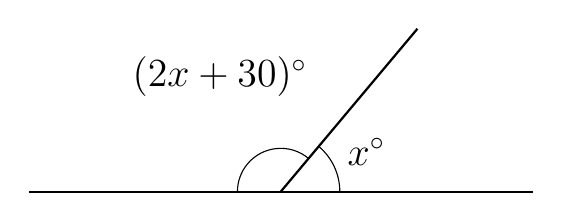
\begin{tikzpicture}[font=\Large]
     \draw[thick] (-3.2,0) -- (3.2,0);
     \draw[thick] (0,0) -- (50:2.7);
     \draw (0.75,0) arc (0:50:0.75);
     \draw (50:0.55) arc (50:180:0.55);
     \node at (25:1.2) {$x^{\circ}$};
     \node at (118:1.65) {$(2x+30)^{\circ}$};
   \end{tikzpicture}}
  {Angles on a straight line add up to $180^{\circ}$.
   \par\vspace{0.3em}
   \steps{$x+2x+30$ & $180$ & \\
          $3x+30$ & $180$ & \by{collect like terms}\\
          $3x$ & $150$ & \by{subtract $30$ from both sides}\\
          $x$ & $50$ & \by{divide both sides by $3$}}}

\qq[\LARGE][\Large]{Find the value of $x$\\[0.5em]
   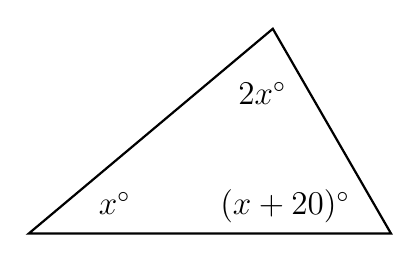
\begin{tikzpicture}[scale=1.15, font=\large]
     \draw[thick] (0,0) -- (4,0) -- (2.695,2.261) -- cycle;
     \node at (0.95,0.33) {$x^{\circ}$};
     \node at (2.83,0.3) {$(x+20)^{\circ}$};
     \node at (2.58,1.55) {$2x^{\circ}$};
   \end{tikzpicture}}
  {The angles in a triangle add up to $180^{\circ}$.
   \par\vspace{0.3em}
   \steps{$x+(x+20)+2x$ & $180$ & \\
          $4x+20$ & $180$ & \by{collect like terms}\\
          $4x$ & $160$ & \by{subtract $20$ from both sides}\\
          $x$ & $40$ & \by{divide both sides by $4$}}}

\qq[\LARGE][\Large]{Amir is $4$ years older than Beth.\\[0.3em]
   The sum of their ages is $30$.\\[0.3em]
   How old is Beth?}
  {We write $b$ for Beth's age in years, so Amir is $b+4$ years old.
   \par\vspace{0.3em}
   \side[0.58]{\steps{$b+(b+4)$ & $30$ & \\
                      $2b+4$ & $30$ & \by{collect like terms}\\
                      $2b$ & $26$ & \by{subtract $4$}\\
                      $b$ & $13$ & \by{divide by $2$}}\\[0.4em]
               Beth is $13$ years old.}
     {\barmodel[0.16]{30}{13/b/\bp,13/b/\bp,4/4/\bp}}}

\qq[\LARGE][\Large]{The sum of three consecutive odd numbers is $75$.\\[0.3em]
   Find the three numbers.}
  {We write $n$ for the smallest number. Consecutive odd numbers differ
   by $2$, so the others are $n+2$ and $n+4$.
   \par\vspace{0.3em}
   \steps{$n+(n+2)+(n+4)$ & $75$ & \\
          $3n+6$ & $75$ & \by{collect like terms}\\
          $3n$ & $69$ & \by{subtract $6$ from both sides}\\
          $n$ & $23$ & \by{divide both sides by $3$}}\\[0.4em]
   The numbers are $23$, $25$ and $27$.}

\qq[\LARGE][\Large]{\side[0.55]{The perimeter of this\\[0.2em]
     rectangle is $32$\,cm.\\[0.4em] Find the value of $x$.}
   {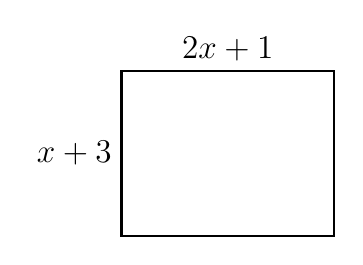
\begin{tikzpicture}[x=0.3cm, y=0.3cm, font=\large]
      \draw[thick] (0,0) rectangle (9,7);
      \node[above] at (4.5,7) {$2x+1$};
      \node[left] at (0,3.5) {$x+3$};
    \end{tikzpicture}}}
  {\steps{$2(2x+1)+2(x+3)$ & $32$ & \\
          $4x+2+2x+6$ & $32$ & \by{expand the brackets}\\
          $6x+8$ & $32$ & \by{collect like terms}\\
          $6x$ & $24$ & \by{subtract $8$ from both sides}\\
          $x$ & $4$ & \by{divide both sides by $6$}}}

\qq[\LARGE][\Large]{\side[0.55]{The perimeter of this\\[0.2em]
     isosceles triangle is $37$\,cm.\\[0.4em] Find the value of $x$.}
   {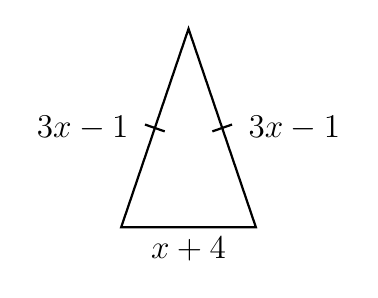
\begin{tikzpicture}[x=0.19cm, y=0.19cm, font=\large]
      \draw[thick] (0,0) -- (9,0) -- (4.5,13.26) -- cycle;
      \node[left=6pt] at (2.25,6.63) {$3x-1$};
      \node[right=6pt] at (6.75,6.63) {$3x-1$};
      \node[below] at (4.5,0) {$x+4$};
      \draw[thick] (1.59,6.86) -- (2.91,6.40);
      \draw[thick] (6.09,6.40) -- (7.41,6.86);
    \end{tikzpicture}}}
  {The perimeter is the total of all three sides.
   \par\vspace{0.3em}
   \steps{$2(3x-1)+(x+4)$ & $37$ & \\
          $7x+2$ & $37$ & \by{expand and collect like terms}\\
          $7x$ & $35$ & \by{subtract $2$ from both sides}\\
          $x$ & $5$ & \by{divide both sides by $7$}}}

\qq[\LARGE][\Large]{I think of a number. Multiplying it by $5$ and\\[0.1em]
   subtracting $3$ gives the same answer as\\[0.1em]
   doubling it and adding $12$. What is my number?}
  {We write $n$ for my number.
   \par\vspace{0.3em}
   \steps{$5n-3$ & $2n+12$ & \\
          $3n-3$ & $12$ & \by{subtract $2n$ from both sides}\\
          $3n$ & $15$ & \by{add $3$ to both sides}\\
          $n$ & $5$ & \by{divide both sides by $3$}}\\[0.4em]
   Check: $5\times 5-3=22$ and $2\times 5+12=22$}

\qq[\Large][\Large]{\side[0.62]{A square has sides of length $x+2$.\\[0.2em]
     An equilateral triangle has sides\\[0.1em] of length $2x-1$.\\[0.2em]
     They have the same perimeter.\\[0.2em] Find the value of $x$.}
   {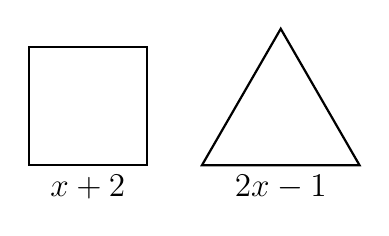
\begin{tikzpicture}[x=0.2cm, y=0.2cm, font=\large]
      \draw[thick] (0,0) rectangle (7.5,7.5);
      \node[below] at (3.75,0) {$x+2$};
      \draw[thick] (11,0) -- (21,0) -- (16,8.66) -- cycle;
      \node[below] at (16,0) {$2x-1$};
    \end{tikzpicture}}}
  {\steps{$4(x+2)$ & $3(2x-1)$ & \\
          $4x+8$ & $6x-3$ & \by{expand the brackets}\\
          $8$ & $2x-3$ & \by{subtract $4x$ from both sides}\\
          $11$ & $2x$ & \by{add $3$ to both sides}\\
          $5.5$ & $x$ & \by{divide both sides by $2$}}}

\qq[\LARGE][\Large]{Write an equation with the unknown on both sides\\[0.3em]
   whose solution is $x=3$}
  {There are many answers. For example, when $x=3$,
   $5x=15$ and $2x+9=15$, so
   \par\vspace{0.3em}
   $5x=2x+9$\\[0.4em]
   Check any answer by substituting $x=3$ into both sides:
   the two sides must be equal.}

%================================================================
\qtopic{Equations with the unknown in the denominator}
%================================================================

\tf{The solution of $\dfrac{12}{x}=3$ is $x=36$}
  {\textbf{False.} $\dfrac{12}{36}=\dfrac{1}{3}$, not $3$.
   \par\vspace{0.4em}
   \steps{$\dfrac{12}{x}$ & $3$ & \\[0.95em]
          $12$ & $3x$ & \by{multiply both sides by $x$}\\
          $4$ & $x$ & \by{divide both sides by $3$}}}

\tf{To solve $\dfrac{20}{x}=5$, we can start by\\[0.3em]
   multiplying both sides by $x$}
  {\textbf{True.} This removes $x$ from the denominator.
   \par\vspace{0.4em}
   \steps{$\dfrac{20}{x}$ & $5$ & \\[0.95em]
          $20$ & $5x$ & \by{multiply both sides by $x$}\\
          $4$ & $x$ & \by{divide both sides by $5$}}}

\tf{$\dfrac{6}{x}=2$ and $\dfrac{x}{6}=2$ have the same solution}
  {\textbf{False.}\\[0.3em]
   $\dfrac{6}{x}=2$ gives $6=2x$, so $x=3$.\\[0.5em]
   $\dfrac{x}{6}=2$ gives $x=12$.}

\tf{The solution of $\dfrac{10}{x}=4$ is $x=2.5$}
  {\textbf{True.} Check: $10\div 2.5=4$\\[0.3em]
   The solution is not $0.4$ or $40$, because $10\div 0.4=25$ and
   $10\div 40=0.25$.
   \par\vspace{0.4em}
   \steps{$\dfrac{10}{x}$ & $4$ & \\[0.95em]
          $10$ & $4x$ & \by{multiply both sides by $x$}\\
          $2.5$ & $x$ & \by{divide both sides by $4$}}}

\tf{The solution of $\dfrac{5}{x}=0$ is $x=0$}
  {\textbf{False.} Dividing by $0$ is not defined, so $x$ cannot be $0$.\\[0.3em]
   Multiplying both sides by $x$ gives $5=0$, which is never true.\\[0.3em]
   The equation has no solution.}

\qq[\Huge][\Large]{Solve $\dfrac{15}{x}=5$}
  {\steps{$\dfrac{15}{x}$ & $5$ & \\[0.95em]
          $15$ & $5x$ & \by{multiply both sides by $x$}\\
          $3$ & $x$ & \by{divide both sides by $5$}}
   \par\vspace{0.6em}
   \barmodel[0.4]{15}{3/x/\bp,3/x/\bp,3/x/\bp,3/x/\bp,3/x/\bp}}

\qq[\Huge][\Large]{Solve $\dfrac{35}{x}=7$}
  {\steps{$\dfrac{35}{x}$ & $7$ & \\[0.95em]
          $35$ & $7x$ & \by{multiply both sides by $x$}\\
          $5$ & $x$ & \by{divide both sides by $7$}}}

\qq[\Huge][\Large]{Solve $\dfrac{18}{x}=4$}
  {\steps{$\dfrac{18}{x}$ & $4$ & \\[0.95em]
          $18$ & $4x$ & \by{multiply both sides by $x$}\\
          $4.5$ & $x$ & \by{divide both sides by $4$}}}

\qq[\Huge][\Large]{Solve $\dfrac{8}{x}=-2$}
  {\steps{$\dfrac{8}{x}$ & $-2$ & \\[0.95em]
          $8$ & $-2x$ & \by{multiply both sides by $x$}\\
          $-4$ & $x$ & \by{divide both sides by $-2$}}\\[0.4em]
   Check: $8\div(-4)=-2$}

\qq[\Huge][\Large]{Solve $\dfrac{12}{x}+1=5$}
  {\steps{$\dfrac{12}{x}+1$ & $5$ & \\[0.95em]
          $\dfrac{12}{x}$ & $4$ & \by{subtract $1$ from both sides}\\[0.95em]
          $12$ & $4x$ & \by{multiply both sides by $x$}\\
          $3$ & $x$ & \by{divide both sides by $4$}}}

\qq[\Huge][\Large]{Solve $\dfrac{20}{x}-3=1$}
  {\steps{$\dfrac{20}{x}-3$ & $1$ & \\[0.95em]
          $\dfrac{20}{x}$ & $4$ & \by{add $3$ to both sides}\\[0.95em]
          $20$ & $4x$ & \by{multiply both sides by $x$}\\
          $5$ & $x$ & \by{divide both sides by $4$}}}

\qq[\Huge][\Large]{Solve $\dfrac{30}{x+1}=6$}
  {\steps{$\dfrac{30}{x+1}$ & $6$ & \\[0.95em]
          $30$ & $6(x+1)$ & \by{multiply both sides by $(x+1)$}\\
          $5$ & $x+1$ & \by{divide both sides by $6$}\\
          $4$ & $x$ & \by{subtract $1$ from both sides}}}

\qq[\Huge][\Large]{Solve $\dfrac{21}{2x+1}=3$}
  {\steps{$\dfrac{21}{2x+1}$ & $3$ & \\[0.95em]
          $21$ & $3(2x+1)$ & \by{multiply both sides by $(2x+1)$}\\
          $7$ & $2x+1$ & \by{divide both sides by $3$}\\
          $6$ & $2x$ & \by{subtract $1$ from both sides}\\
          $3$ & $x$ & \by{divide both sides by $2$}}}

\qq[\Huge][\Large]{Solve $\dfrac{6}{x}=\dfrac{3}{4}$}
  {\steps{$\dfrac{6}{x}$ & $\dfrac{3}{4}$ & \\[0.95em]
          $24$ & $3x$ & \by{multiply both sides by $4x$}\\
          $8$ & $x$ & \by{divide both sides by $3$}}\\[0.4em]
   Check: $\dfrac{6}{8}=\dfrac{3}{4}$}

\qq[\Large][\Large]{A train travels $240$\,km at an average speed of $80$\,km/h.\\[0.4em]
   Use $\text{speed}=\dfrac{\text{distance}}{\text{time}}$ to write an equation
   for the time,\\[0.6em] $t$ hours, and solve it.}
  {\steps{$\dfrac{240}{t}$ & $80$ & \\[0.95em]
          $240$ & $80t$ & \by{multiply both sides by $t$}\\
          $3$ & $t$ & \by{divide both sides by $80$}}\\[0.4em]
   The journey takes $3$ hours.}

%================================================================
\qtopic{Equations with algebraic fractions}
%================================================================

\tf{To solve $\dfrac{x}{2}+\dfrac{x}{3}=5$ we can multiply every term by $6$}
  {\textbf{True.} $6$ is a common multiple of $2$ and $3$,\\
   so multiplying by $6$ clears both fractions.
   \par\vspace{0.4em}
   \steps{$\dfrac{x}{2}+\dfrac{x}{3}$ & $5$ & \\[0.95em]
          $3x+2x$ & $30$ & \by{multiply every term by $6$}\\
          $5x$ & $30$ & \by{collect like terms}\\
          $x$ & $6$ & \by{divide both sides by $5$}}}

\tf{Multiplying $\dfrac{x}{4}+1=\dfrac{x}{2}$ by $4$ gives $x+1=2x$}
  {\textbf{False.} Every term is multiplied by $4$, including the $1$.
   \par\vspace{0.4em}
   \steps{$\dfrac{x}{4}+1$ & $\dfrac{x}{2}$ & \\[0.95em]
          $x+4$ & $2x$ & \by{multiply every term by $4$}\\
          $4$ & $x$ & \by{subtract $x$ from both sides}}}

\tf{$\dfrac{x+1}{2}=\dfrac{x+4}{3}$ gives $3(x+1)=2(x+4)$}
  {\textbf{True.} Multiplying both sides by $6$ clears both fractions.
   \par\vspace{0.4em}
   \steps{$3(x+1)$ & $2(x+4)$ & \\
          $3x+3$ & $2x+8$ & \by{expand the brackets}\\
          $x$ & $5$ & \by{subtract $2x$ and $3$ from both sides}}}

\tf[\Large][\Large]{Multiplying $\dfrac{x}{3}-\dfrac{x-2}{4}=1$ by $12$ gives\\[0.7em]
   $4x-3x-6=12$}
  {\textbf{False.} The minus sign applies to the whole of $3(x-2)$, so
   $-3\times(-2)=+6$.
   \par\vspace{0.4em}
   \steps{$4x-3(x-2)$ & $12$ & \\
          $4x-3x+6$ & $12$ & \by{expand the bracket}\\
          $x$ & $6$ & \by{collect like terms and subtract $6$}}}

\tf{The solution of $\dfrac{2}{x}=\dfrac{3}{x+1}$ is $x=2$}
  {\textbf{True.} Check: $\dfrac{2}{2}=1$ and $\dfrac{3}{2+1}=1$
   \par\vspace{0.4em}
   \steps{$2(x+1)$ & $3x$ & \by{multiply both sides by $x(x+1)$}\\
          $2x+2$ & $3x$ & \by{expand the bracket}\\
          $2$ & $x$ & \by{subtract $2x$ from both sides}}}

\qq[\Huge][\Large]{Solve $\dfrac{x}{2}+\dfrac{x}{4}=6$}
  {\steps{$\dfrac{x}{2}+\dfrac{x}{4}$ & $6$ & \\[0.95em]
          $2x+x$ & $24$ & \by{multiply every term by $4$}\\
          $3x$ & $24$ & \by{collect like terms}\\
          $x$ & $8$ & \by{divide both sides by $3$}}}

\qq[\Huge][\Large]{Solve $\dfrac{x}{2}-\dfrac{x}{5}=3$}
  {\steps{$\dfrac{x}{2}-\dfrac{x}{5}$ & $3$ & \\[0.95em]
          $5x-2x$ & $30$ & \by{multiply every term by $10$}\\
          $3x$ & $30$ & \by{collect like terms}\\
          $x$ & $10$ & \by{divide both sides by $3$}}}

\qq[\Huge][\Large]{Solve $\dfrac{x+2}{3}=\dfrac{x-1}{2}$}
  {\steps{$\dfrac{x+2}{3}$ & $\dfrac{x-1}{2}$ & \\[0.95em]
          $2(x+2)$ & $3(x-1)$ & \by{multiply both sides by $6$}\\
          $2x+4$ & $3x-3$ & \by{expand the brackets}\\
          $7$ & $x$ & \by{subtract $2x$ and add $3$}}}

\qq[\Huge][\Large]{Solve $\dfrac{x+1}{2}+\dfrac{x+3}{4}=5$}
  {\steps{$\dfrac{x+1}{2}+\dfrac{x+3}{4}$ & $5$ & \\[0.95em]
          $2(x+1)+(x+3)$ & $20$ & \by{multiply every term by $4$}\\
          $3x+5$ & $20$ & \by{expand and collect like terms}\\
          $3x$ & $15$ & \by{subtract $5$ from both sides}\\
          $x$ & $5$ & \by{divide both sides by $3$}}}

\qq[\Huge][\Large]{Solve $\dfrac{2x+2}{3}-\dfrac{x-1}{4}=3$}
  {The minus sign applies to the whole of $3(x-1)$.
   \par\vspace{0.3em}
   \steps{$4(2x+2)-3(x-1)$ & $36$ & \by{multiply every term by $12$}\\
          $8x+8-3x+3$ & $36$ & \by{expand the brackets}\\
          $5x+11$ & $36$ & \by{collect like terms}\\
          $5x$ & $25$ & \by{subtract $11$ from both sides}\\
          $x$ & $5$ & \by{divide both sides by $5$}}}

\qq[\Huge][\Large]{Solve $\dfrac{4}{x}+\dfrac{1}{2x}=3$}
  {\steps{$\dfrac{4}{x}+\dfrac{1}{2x}$ & $3$ & \\[0.95em]
          $8+1$ & $6x$ & \by{multiply every term by $2x$}\\
          $9$ & $6x$ & \by{collect like terms}\\
          $1.5$ & $x$ & \by{divide both sides by $6$}}}

\qq[\Huge][\Large]{Solve $\dfrac{3}{x+1}=\dfrac{2}{x-1}$}
  {\steps{$\dfrac{3}{x+1}$ & $\dfrac{2}{x-1}$ & \\[0.95em]
          $3(x-1)$ & $2(x+1)$ & \by{multiply both sides by $(x+1)(x-1)$}\\
          $3x-3$ & $2x+2$ & \by{expand the brackets}\\
          $x$ & $5$ & \by{subtract $2x$ and add $3$}}\\[0.4em]
   Check: $\dfrac{3}{6}=\dfrac{1}{2}$ and $\dfrac{2}{4}=\dfrac{1}{2}$}

\qq[\Huge][\Large]{Solve $x+\dfrac{6}{x}=5$}
  {\steps{$x+\dfrac{6}{x}$ & $5$ & \\[0.95em]
          $x^{2}+6$ & $5x$ & \by{multiply every term by $x$}\\
          $x^{2}-5x+6$ & $0$ & \by{subtract $5x$ from both sides}\\
          $(x-2)(x-3)$ & $0$ & \by{factorise}}\\[0.4em]
   $x=2$ or $x=3$}

\qq[\Huge][\Large]{Solve $\dfrac{6}{x}-\dfrac{6}{x+1}=1$}
  {\steps{$6(x+1)-6x$ & $x(x+1)$ & \by{multiply every term by $x(x+1)$}\\
          $6$ & $x^{2}+x$ & \by{expand and collect like terms}\\
          $0$ & $x^{2}+x-6$ & \by{subtract $6$ from both sides}\\
          $0$ & $(x+3)(x-2)$ & \by{factorise}}\\[0.4em]
   $x=-3$ or $x=2$}

\qq[\LARGE][\Large]{Write an equation with two algebraic fractions\\[0.3em]
   whose solution is $x=4$}
  {There are many answers. We choose the fractions,\\
   then work out the right-hand side using $x=4$. For example,
   \par\vspace{0.4em}
   $\dfrac{x+2}{3}+\dfrac{x}{2}=4$\\[0.5em]
   Check: $\dfrac{4+2}{3}+\dfrac{4}{2}=2+2=4$}

%================================================================
\qtopic{Simultaneous equations}
%================================================================

\tf{$x=3$, $y=2$ is the solution of\\[0.3em]
   $x+y=5$ and $x-y=1$}
  {\textbf{True.} The values fit both equations:\\[0.3em]
   $3+2=5$ and $3-2=1$}

\tf{$x=4$, $y=1$ is the solution of\\[0.3em]
   $x+y=5$ and $2x+y=7$}
  {\textbf{False.} The values fit the first equation,\\
   but $2\times 4+1=9$, not $7$.\\[0.3em]
   The solution has to fit both equations. It is $x=2$, $y=3$:\\[0.3em]
   $2+3=5$ and $2\times 2+3=7$}

\tf{To eliminate $y$ from\\[0.3em]
   $3x+2y=16$ and $x+2y=8$\\[0.3em]
   we add the equations}
  {\textbf{False.} Both $y$ terms are $+2y$, so we subtract.
   \par\vspace{0.4em}
   \simwork{\by{(1)} & $3x+2y$ & $16$\\
            \by{(2)} & $x+2y$ & $8$\\
            \by{(1) $-$ (2)} & $2x$ & $8$}\\[0.3em]
   $x=4$, and then $4+2y=8$ gives $y=2$.}

\tf[\Large][\Large]{The solution of a pair of linear simultaneous equations\\[0.2em]
   is given by the point where their graphs cross}
  {\side[0.52]{\textbf{True.} The point $(2,3)$ is on both lines,
     so $x=2$, $y=3$ fits both equations.\\[0.4em]
     $2+3=5$ and $3=2+1$}
   {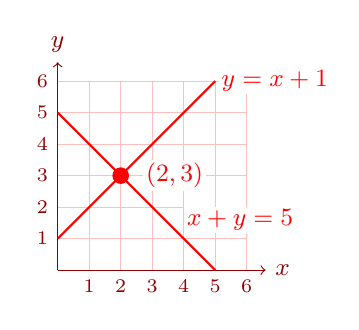
\begin{tikzpicture}[x=0.4cm, y=0.4cm, font=\small]
      \draw[red!25, step=1] (0,0) grid (6,6);
      \draw[->, red!55!black] (0,0) -- (6.6,0) node[right] {$x$};
      \draw[->, red!55!black] (0,0) -- (0,6.6) node[above] {$y$};
      \foreach \i in {1,...,6} {
        \node[below, red!55!black, font=\scriptsize] at (\i,0) {$\i$};
        \node[left, red!55!black, font=\scriptsize] at (0,\i) {$\i$};}
      \draw[red, thick] (0,5) -- (5,0);
      \draw[red, thick] (0,1) -- (5,6);
      \node[red, right, fill=white, inner sep=1pt] at (5.1,6) {$y=x+1$};
      \node[red, right, fill=white, inner sep=1pt] at (4.0,1.6) {$x+y=5$};
      \fill[red] (2,3) circle (3pt);
      \node[red, right=8pt, fill=white, inner sep=1pt] at (2,3) {$(2,3)$};
    \end{tikzpicture}}}

\tf{To eliminate $x$ from\\[0.3em]
   $2x+3y=12$ and $x+y=5$\\[0.3em]
   we can multiply the second equation by $2$}
  {\textbf{True.} This makes the $x$ terms the same.
   \par\vspace{0.4em}
   \simwork{\by{(1)} & $2x+3y$ & $12$\\
            \by{(2) $\times 2$} & $2x+2y$ & $10$\\
            \by{(1) $-$ (2) $\times 2$} & $y$ & $2$}\\[0.3em]
   Then $x+2=5$ gives $x=3$.}

\qq[\Huge][\Large]{Solve\\[0.3em]
   $\begin{aligned} x+y&=10\\ x-y&=4 \end{aligned}$}
  {\simwork{\by{(1)} & $x+y$ & $10$\\
            \by{(2)} & $x-y$ & $4$\\
            \by{(1) $+$ (2)} & $2x$ & $14$}\\[0.3em]
   $x=7$, and then $7+y=10$ gives $y=3$.}

\qq[\Huge][\Large]{Solve\\[0.3em]
   $\begin{aligned} 2x+y&=11\\ x+y&=7 \end{aligned}$}
  {\simwork{\by{(1)} & $2x+y$ & $11$\\
            \by{(2)} & $x+y$ & $7$\\
            \by{(1) $-$ (2)} & $x$ & $4$}\\[0.3em]
   Then $4+y=7$ gives $y=3$.}

\qq[\Huge][\Large]{Solve\\[0.3em]
   $\begin{aligned} 3x+2y&=13\\ x-2y&=-1 \end{aligned}$}
  {The $y$ terms have opposite signs, so we add.
   \par\vspace{0.3em}
   \simwork{\by{(1)} & $3x+2y$ & $13$\\
            \by{(2)} & $x-2y$ & $-1$\\
            \by{(1) $+$ (2)} & $4x$ & $12$}\\[0.3em]
   $x=3$, and then $9+2y=13$ gives $y=2$.}

\qq[\Huge][\Large]{Solve\\[0.3em]
   $\begin{aligned} 5x+2y&=24\\ 3x+2y&=16 \end{aligned}$}
  {The $y$ terms are the same, so we subtract.
   \par\vspace{0.3em}
   \simwork{\by{(1)} & $5x+2y$ & $24$\\
            \by{(2)} & $3x+2y$ & $16$\\
            \by{(1) $-$ (2)} & $2x$ & $8$}\\[0.3em]
   $x=4$, and then $20+2y=24$ gives $y=2$.}

\qq[\LARGE][\Large]{Solve\\[0.3em]
   $\begin{aligned} y&=2x+1\\ x+y&=7 \end{aligned}$}
  {\side[0.58]{We substitute $y=2x+1$\\ into the second equation.\\[0.4em]
              \steps{$x+(2x+1)$ & $7$ & \\
                     $3x+1$ & $7$ & \by{collect like terms}\\
                     $3x$ & $6$ & \by{subtract $1$}\\
                     $x$ & $2$ & \by{divide by $3$}}\\[0.4em]
              Then $y=2\times 2+1=5$.}
     {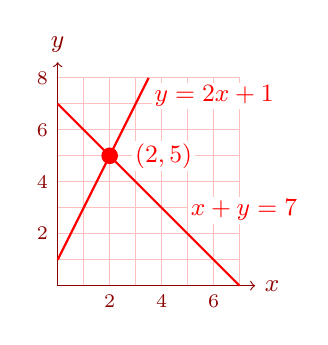
\begin{tikzpicture}[x=0.33cm, y=0.33cm, font=\small]
        \draw[red!25, step=1] (0,0) grid (7,8);
        \draw[->, red!55!black] (0,0) -- (7.6,0) node[right] {$x$};
        \draw[->, red!55!black] (0,0) -- (0,8.6) node[above] {$y$};
        \foreach \i in {2,4,6} {
          \node[below, red!55!black, font=\scriptsize] at (\i,0) {$\i$};}
        \foreach \i in {2,4,6,8} {
          \node[left, red!55!black, font=\scriptsize] at (0,\i) {$\i$};}
        \draw[red, thick] (0,1) -- (3.5,8);
        \draw[red, thick] (0,7) -- (7,0);
        \node[red, right, fill=white, inner sep=1pt] at (3.6,7.3) {$y=2x+1$};
        \node[red, right, fill=white, inner sep=1pt] at (5.0,2.9) {$x+y=7$};
        \fill[red] (2,5) circle (3pt);
        \node[red, right=8pt, fill=white, inner sep=1pt] at (2,5) {$(2,5)$};
      \end{tikzpicture}}}

\qq[\Huge][\Large]{Solve\\[0.3em]
   $\begin{aligned} 2x+3y&=13\\ x+y&=5 \end{aligned}$}
  {\simwork{\by{(1)} & $2x+3y$ & $13$\\
            \by{(2) $\times 2$} & $2x+2y$ & $10$\\
            \by{(1) $-$ (2) $\times 2$} & $y$ & $3$}\\[0.3em]
   Then $x+3=5$ gives $x=2$.}

\qq[\Huge][\Large]{Solve\\[0.3em]
   $\begin{aligned} 3x+2y&=17\\ 2x-y&=9 \end{aligned}$}
  {\simwork{\by{(1)} & $3x+2y$ & $17$\\
            \by{(2) $\times 2$} & $4x-2y$ & $18$\\
            \by{(1) $+$ (2) $\times 2$} & $7x$ & $35$}\\[0.3em]
   $x=5$, and then $10-y=9$ gives $y=1$.}

\qq[\Huge][\Large]{Solve\\[0.3em]
   $\begin{aligned} 3x+4y&=25\\ 2x+3y&=18 \end{aligned}$}
  {\simwork{\by{(1) $\times 2$} & $6x+8y$ & $50$\\
            \by{(2) $\times 3$} & $6x+9y$ & $54$\\
            \by{(2) $\times 3$ $-$ (1) $\times 2$} & $y$ & $4$}\\[0.3em]
   Then $3x+16=25$ gives $x=3$.}

\qq[\Large][\Large]{$2$ coffees and $3$ teas cost \pounds$9.10$.\\[0.3em]
   $1$ coffee and $2$ teas cost \pounds$5.20$.\\[0.3em]
   Find the cost of one coffee and the cost of one tea.}
  {We work in pence, and write $c$ for the cost of one coffee\\
   and $t$ for the cost of one tea.
   \par\vspace{0.3em}
   \simwork{\by{(1)} & $2c+3t$ & $910$\\
            \by{(2)} & $c+2t$ & $520$\\
            \by{(2) $\times 2$} & $2c+4t$ & $1040$\\
            \by{(2) $\times 2$ $-$ (1)} & $t$ & $130$}\\[0.3em]
   Then $c+260=520$ gives $c=260$. A coffee costs \pounds$2.60$\\
   and a tea costs \pounds$1.30$.}

\qq[\LARGE][\Large]{Write a pair of simultaneous equations\\[0.3em]
   whose solution is $x=4$, $y=-1$}
  {There are many answers. We choose the left-hand sides,\\
   then work out the right-hand sides using $x=4$ and $y=-1$.\\
   For example,
   \par\vspace{0.3em}
   $\begin{aligned} x+y&=3\\ 2x-y&=9 \end{aligned}$\\[0.4em]
   Check: $4+(-1)=3$ and $2\times 4-(-1)=9$}

\end{document}
